\documentclass{standalone}
\usepackage{tikz}
\usepackage{ctex,siunitx}
\usepackage{tkz-euclide}
\usepackage{amsmath}
\usetikzlibrary{patterns, calc}
\usetikzlibrary {decorations.pathmorphing, decorations.markings, decorations.shapes,}
\tikzset{
pencil/.pic={
  \fill[left color =green!80!black,right color=green!80!black,middle color=white](-0.05,0)rectangle(0.05,1.5);
  \fill(-0.05,1.5)--(0,1.7)--(0.05,1.5);
  \fill[left color =brown,right color=brown,middle color=white](-0.05,1.5)--(-0.02,1.62)--(0.02,1.62)--(0.05,1.5);
}
}
\begin{document}
\small
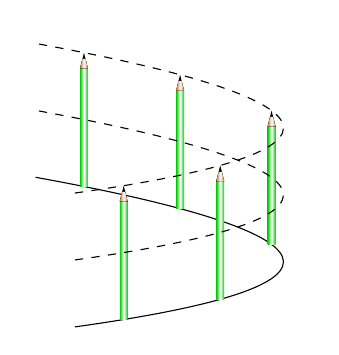
\begin{tikzpicture}[decoration={markings,
  mark=between positions 0.1 and 1 step 0.2 with
  {\pic {pencil};}}]
  \useasboundingbox (-0.6,0)rectangle(3,3.8);
  \draw[postaction={decorate}](0,0)..controls(4.3,0.6)and(2.8,1.3)..(-0.5,1.9);
  \draw[thin,dashed](0,0.85)..controls(4.3,1.45)and(2.8,2.15)..(-0.5,2.75);
  \draw[thin,dashed](0,1.7)..controls(4.3,2.3)and(2.8,3.0)..(-0.5,3.6);
\end{tikzpicture}
\end{document}